\documentclass{article}

% Packages for additional functionality
\usepackage{amsmath} % For mathematical equations
\usepackage{graphicx} % For including images
\usepackage{hyperref} % For hyperlinks
\usepackage{float}

\newcommand{\para}{\vspace{8pt}} % New paragraph command

\setlength{\parindent}{0pt} % No indentation for new paragraphs

\begin{document}
\title{Optimal Hedging with Advanced Delta Modelling }
\author{Joseph Kirk}
\date{\today}

\maketitle

\newpage
\tableofcontents

\newpage
\section{Introduction}

\subsection{Preamble}
This report is prepared to satisfy the requirements of the CQF assignment \textit{Optimal Hedging with Advanced Delta Modelling}. Three topics are studied.

\para
The first investigation uses Geometric Brownian Motion as an example to introduce Monte Carlo methods and variance reduction techniques. 
Specifically we study the effect of antithetic variates, sobol sequences and the brownian bridge to reduce the number of paths required to converge on the Black Scholes 
price of a European Call Option.

\para
The second study looks at the affect of hedging with actual and implied volatility under the condition that future realised volatility is
above implied volatility.  We demonstrate through simulation and prove with mathematical workings that hedging with the actual volatility leads to a known value of total 
P\&L.  

\para
We conclude the report by partially replicating the study conducted by John C. Hull and Alan White \cite{hull}. Using 2023 implied volatility for SPX options (provided by OptionsDX)
we fit the minimum variance delta (MVD) model. This model anticipates the change in magnitude of implied volatility and applies a correction to the Black Scholes delta.

\subsection{Code}

The Python code used to generate the data and plots has been provided alongside this report. Core functionality has been coded as reusable modules and the experiments
are available as Jupyter notebooks. Jupyter has been used because it is easy to generate plots.

TODO: Add a table detailing the functions have been implemented

\newpage

\section{Monte Carlo Variance Reduction}

Monte Carlo methods are a class of computational algorithms that rely on repeated random sampling to obtain numerical results. It is particularly prevelant in the field of finance
where many financial models do not have closed form solutions. While European options can be priced using the Black-Scholes formula (which is derived from Geometric Brownian Motion), more complex 
products such as American options, that can be exercised at any point, require a numerical approach. 

\para
To price an option using Monte Carlo methods we must compute the fair value of said option. This is the present value of the expected payoff at expiry under a risk-neutral random walk. 

\begin{enumerate}
    \item Simulate the risk-neutral random walk starting at today's value of the asset S0 over the required time horizon. This gives one realization of the underlying price path.
    \item For this realization calculate the option payoff.
    \item Perform many more such realizations over the time horizon.
    \item Calculate the average payoff over all realizations.
    \item Take the present value of this average, this is the option value.
\end{enumerate}

Monte Carlo is a widely accepted method for pricing options since it is simple to implement and can be used for products with complex path dependency. However, it can be computationally expensive.  If we 
can reduce the variance of the simulated path then we can reduce the number of paths we need to calculate. This is the aim of variance reduction techniques.  To study variance reduction techniques we use 
the motivating example of pricing a European Call Option whose underlying follows Geometric Brownian Motion. Here is the stochastic differential equation (SDE) for GBM in the risk neutral world. 

\[
dS(t) = r S(t) \, dt + \sigma S(t) \, dW(t)
\]

The analytical solution for GBM is given by

\[
S(t) = S(0) \exp \left( \left( r - \frac{\sigma^2}{2} \right) t + \sigma W(t) \right)
\]

It is possible to generate the asset price at time $T$ using a single step. Since we wish to investigate variance reduction techniques 
we opt to focus our investigation on the numerical solutions discussed in the following section (Euler Maruyama and Milstein). These numerical methods
require the full path to be simulated. Monte carlo simulations using the analytical solution have been provided in the code.

\subsection{Numerical Solutions}

In this section we present numerical schemes for the solution of the GBM SDE. 

\subsubsection{The Euler Scheme}

The Euler-Maruyama discretization is a numerical method used to approximate solutions to stochastic differential equations (SDEs). The Euler-Maruyama method approximates 
the solution of an SDE by discretizing time into small steps of size $\Delta t$. The discretized form of the SDE is given by:

\[
X_{t_{n+1}} = X_{t_n} + a(X_{t_n}, t_n) \Delta t + b(X_{t_n}, t_n) \Delta W_n
\]

where $\Delta W_n = W_{t_{n+1}} - W_{t_n} \sim \mathcal{N}(0, \Delta t)$ is a normally distributed random variable with mean 0 and variance $\Delta t$.

\para
Using the Euler-Maruyama method, the discretized form of GBM is:

\[
S_{t_{n+1}} = S_{t_n} + \mu S_{t_n} \Delta t + \sigma S_{t_n} \Delta W_n
\]

\subsubsection{The Milstein Scheme}

The Milstein scheme improves upon the Euler-Maruyama method by adding a correction term involving the derivative of the diffusion coefficient. 
The discretized form of the SDE using the Milstein scheme is given by:

\[
X_{t_{n+1}} = X_{t_n} + a(X_{t_n}, t_n) \Delta t + b(X_{t_n}, t_n) \Delta W_n + \frac{1}{2} b(X_{t_n}, t_n) \frac{\partial b(X_{t_n}, t_n)}{\partial X} \left( (\Delta W_n)^2 - \Delta t \right)
\]

For GBM, the derivative of the diffusion term $b(S_t, t) = \sigma S_t$ with respect to $S_t$ is $\frac{\partial b(S_t, t)}{\partial S} = \sigma$. Using the Milstein scheme, the discretized form is:

\[
S_{t_{n+1}} = S_{t_n} + \mu S_{t_n} \Delta t + \sigma S_{t_n} \Delta W_n + \frac{1}{2} \sigma S_{t_n} \sigma \left( (\Delta W_n)^2 - \Delta t \right)
\]

\newpage
\subsection{Variance Reduction Techniques}

The accuracy of a Monte Carlo simulation is measured by the standard error $\sigma / \sqrt{N}$. To improve the accuracy of a simulation we can increase the number 
of random paths $N$ or reduce the standard deviation $\sigma$. Variance reduction techniques aim to reduce the standard error by reducing the variance of the simulated paths.

\subsubsection{Antithetic Variates}

Antithetic variates leverage the fact that for every gaussian drawn there is a corresponding negative variate which 
has the same probability of being drawn. If we draw variate $v_i = v(z_i)$ then we also use $v_i' = v(-z_i)$. $v_i'$ 
is negatively correlated to $v_i$ but has the same variance.\cite{jackel}

\[
\text{Var}\left( \frac{v_i + v_i'}{2} \right) = \frac{1}{2} \left( \text{Var}(v_i) + \text{Cov}(v_i, v_i') \right)
\]

Because $v_i$ and $v_i'$ are negatively correlated, $\text{Cov}(v_i, v_i') < 0$.

\[
\text{Var}\left( \frac{v_i + v_i'}{2} \right) < \frac{1}{2} \, \text{Var}(v_i)
\]

\subsubsection{Sobol Sequences}

Sobol sequences are a type of low-discrepancy sequence used in numerical methods for generating quasi-random points. 
Unlike purely random sequences, which can have clusters and gaps, quasi-random sequences like Sobol sequences are designed 
to fill the space more evenly. This results in more reliable and faster convergence in numerical simulations. We illustrate 
the difference between random numbers and sobol sequences in Figure \ref{fig:sobol}.

\begin{figure}[ht]
    \centering
    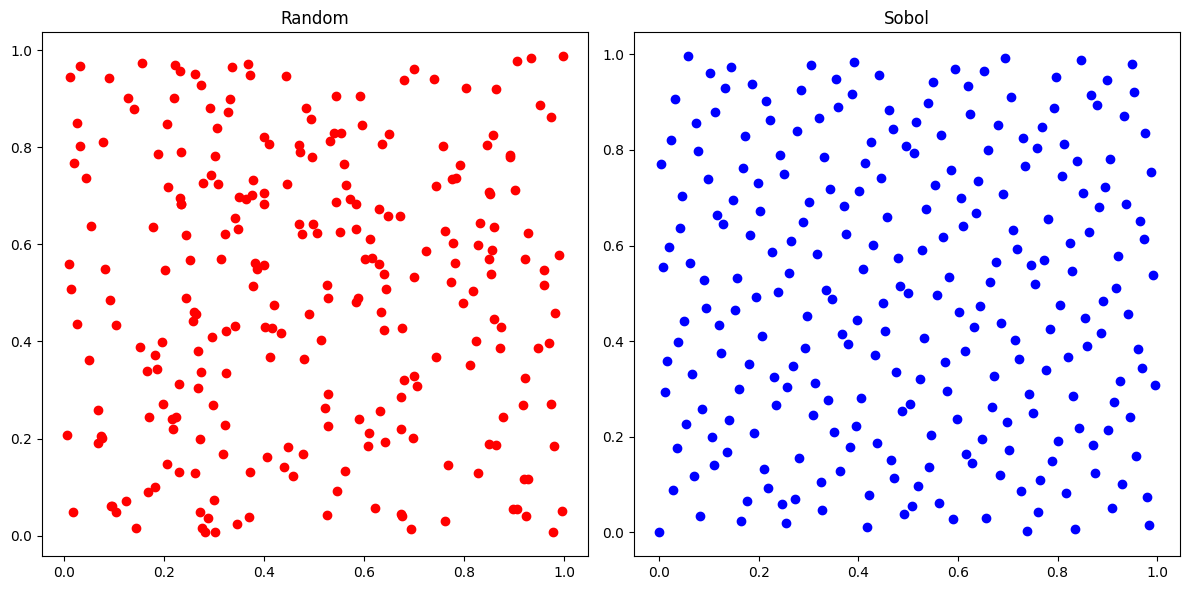
\includegraphics[width=0.8\textwidth]{images/sobol.png}
    \caption{Sobol Sequence}
    \label{fig:sobol}
\end{figure}

\subsubsection{Brownian Bridge}

Brownian Bridge is a path construction method. Rather than building the Wiener path incrementally, the Brownian Bridge uses
the first variate $z_1$ to determine the terminal point $W_{t_n} = \sqrt{t_n}z_1$. The next variate $z_2$ is used to determine a 
point on the path $W_j$ conditional on points $W_{t_n}$ and $W_0=0$. This is repeated until the entire path is constructed. 

\[
W(T) = \sqrt{T}z_1
\]

\[
W(T/2) = \frac{1}{2}W(T/2) + \frac{1}{2}\sqrt{T}z_2
\]

\[
W(T/4) = \frac{1}{2}(W(T/2) + W(T)) + \frac{1}{2}\sqrt{T}z_4
\]

etc. The general formula for the Brownian Bridge is

\[
W(t_i) = (1 - \gamma)(W(t_l)) + \gamma W(t_m) + \sqrt{\gamma(1-\gamma)(m-l)\Delta t}z_i
\]

\para
Incremental and Brownian Bridge path constructions have the same variance so we'd expect a similar rate of convergence. We show in our
results that the Brownian Bridge combined with a Sobol sequence has superior convergence rate. It was suggested my Markowitz\cite{markowitz} 
that the improvement in convergence is due to reduction of the effective dimension of the problem.

\subsection{Results}

In this section we present the results of pricing a European Call Option using the Euler approximation with the following variance reduction / path construction techniques

\begin{itemize}
    \item Antithetic Variates
    \item Sobol Sequences
    \item Brownian Bridge
    \item Sobol Sequences with Brownian Bridge
\end{itemize}

We replicate the workings of Sergei Kucherenko and Nishant Shah \cite{sergei} and use
the following parameters for the simulation: $S_0 = 100$, $K = 100$, $r = 0.05$, $\sigma = 0.2$, $T = 0.5$.
The Black-Scholes price of the option is 6.89.  128 steps are computed and the number of simulations
is varied from 2 to 256.  As expected there is little difference in the convergence rates of incremental and brownian bridge path 
construction in the absence of variance reduction techniques. If we combine the Sobol sequence with the Brownian Bridge we see 
a significant improvement in convergence rate. Figure \ref{fig:option_price} shows the evolution of the price estimate price as the number
simulations is increased.

\begin{figure}[h]
    \centering
    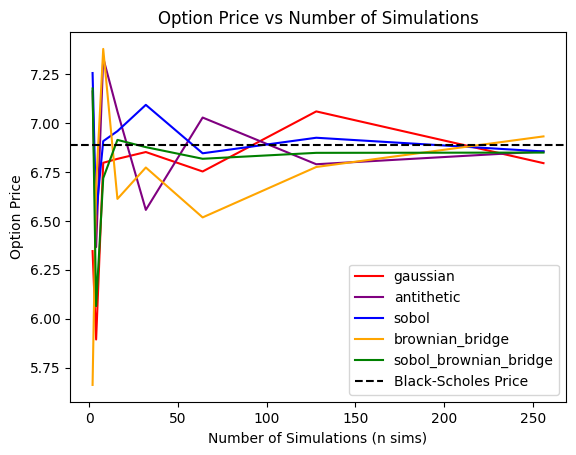
\includegraphics[width=0.8\textwidth]{images/option_price.png}
    \caption{European Call Option Price Convergence}
    \label{fig:option_price}
\end{figure}

\para
We also look at the root mean square error (RMSE). Each simulation is run $L=50$ times.

\[
RMSE = \sqrt{\frac{1}{L} \sum_{l=1}^{L} (V^l - V^{BS})^2}
\]

The RMSE is plotted against the number of simulations in Figure \ref{fig:rmse}. When variance reduction techniques are
applied the accuracy of the results is significantly improved reducing the number of simulations needed to achieve
a desired level of accuracy.  According to the simulations the convergence rate of the Brownian Bridge with Sobol sequences
decreases as $1/N^{0.95}$.

\begin{figure}[h]
    \centering
    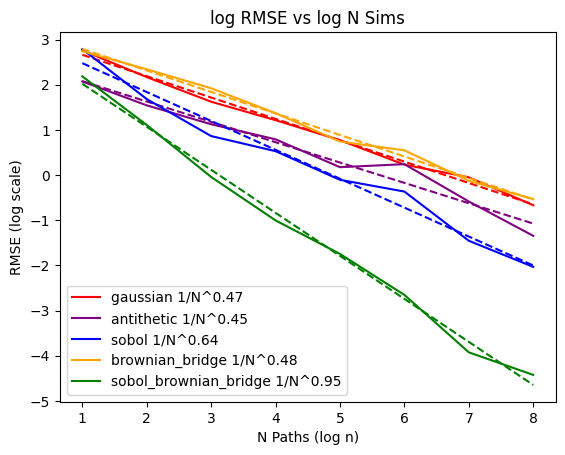
\includegraphics[width=0.8\textwidth]{images/rmse.png}
    \caption{Root mean square error vs the number of simulations}
    \label{fig:rmse}
\end{figure}

\newpage

\section{Hedging with actual volatility}

By hedging with actual volatility we are replicating a short position in a correctly priced option. The payoffs for the long option and the short replicated option will
exactly cancel.

Set up a long option and a short stock portfolio. The option is valued at $V^i$, and we hedge with $-\Delta^a S$ of the stock.
The portfolio is left for a short time period $\delta_t$ and revalued.  In the following notation superscript $a$ refers to actual
and superscript $i$ refers to implied.  Dividends are ignored for brevity, but it is a small extension.

\para
'Today' at time $t$

\begin{table}[H]
    \centering
    \begin{tabular}{|c|c|}
        \hline
        \textbf{Component} & \textbf{Value} \\
        \hline
        Option & $V^{i}$ \\
        \hline
        Stock & $-\Delta^{a}S$ \\
        \hline
        Cash & $-V^{i} + \Delta^{a}S$ \\
        \hline
    \end{tabular}
    \caption{Portfolio at time $t$}
    \label{tab:portfolio_t}
\end{table}

\para
'Tomorrow' at time $t + \delta_t$
\begin{table}[H]
    \centering
    \begin{tabular}{|c|c|}
        \hline
        \textbf{Component} & \textbf{Value} \\
        \hline
        Option & $V^{i}$ \\
        \hline
        Stock & $-\Delta^{a}S$ \\
        \hline
        Cash & $-V^{i} + \Delta^{a}S$ \\
        \hline
    \end{tabular}
    \caption{Portfolio at time $t + \delta_{t}$}
    \label{tab:portfolio_t_plus_delta_t}
\end{table}

Marked to market we have made the following profit over one time step

\begin{center}
\begin{equation}
    dV^i - \Delta^a dS -(V^i - \Delta^a S) rdt
    \label{tab:eq1}
\end{equation}
\end{center}


If the option is priced using the actual volatility then the option is correctly valued at $V^a$ so we can write

\begin{center}
\begin{equation}
    dV^a - \Delta^a dS -(V^a - \Delta^a S) rdt = 0 
    \label{tab:eq2}
\end{equation}
\end{center}

Subtracting \ref{tab:eq1} from \ref{tab:eq2} we can rewrite the mark-to-market profit from $t$ to $t + \delta_t$ as

\begin{center}
\begin{align*}
    \ref{tab:eq1} - \ref{tab:eq2} & = dV^i - dV^a + r(V^a - \Delta^a S) dt - r (V^i - \Delta^a S) dt \\[2pt]
                                  & = dV^i - dV^a + r(V^i - V^a) dt \\[2pt]
                                  & = e^{rt} d(e^{-rt} (V^i - V^a)) \\[2pt]
    d(e^{-rt}V)                   & = d(e^{-rt} dV) -r e^{-rt} V dt \\[2pt]
                                  & = e^{-rt} (dV -rV dt) \\
\end{align*}
\end{center}


The present value of this profit at $t_0$ is

\begin{center}
\begin{equation}
    e^{-r(t-t_0)} e^{rt} d(e^{-rt} (V^i - V^a)) = e^{-rt_0} d(e^{-rt} (V^i - V^a dt))
\end{equation}
\end{center}

So the total profit from $t_0$ to expiration is

\begin{center}
\begin{equation}
    e^{r(t_0)} \int_{t_0}^{T} d(e^{-rt} (V^i - V^a)) = V^a - V^i
\end{equation}
\end{center}


\newpage

\section{Hedging with implied volatility}

\section{Minimum Variance Delta}


\begin{thebibliography}{9}
\bibitem{hull}
J. Hull, A. White. \textit{Optimal delta hedging for options}. 2017
\bibitem{sergei}
S. Kucherenko, N. Shah \textit{The Importance of being Global. Application of Global Sensitivity Analysis in Monte Carlo Option Pricing}.
\bibitem{jackel}
P. J{\"a}ckel \textit{Monte Carlo Methods in Finance}.
\bibitem{markowitz}
B. Moskowitz, R.E. Caflisch. \textit{Smoothness and Dimension Reduction in Quasi-Monte-Carlo}
\end{thebibliography}
\end{document}

